%% ------------------------------------------------------------------------- %%
\chapter{Introdução}
\label{cap:introducao}

Esse trabalho se propõe a ser uma introdução a Aprendizado de Reforço, enviesado para a compreensão de alguns resultados mais recentes na área (?) que, seguindo a tendência de outras áreas dentro de Aprendizado de Máquina (?), utilizam redes neurais para aproximação de funções.

\begin{figure}
    \centering
        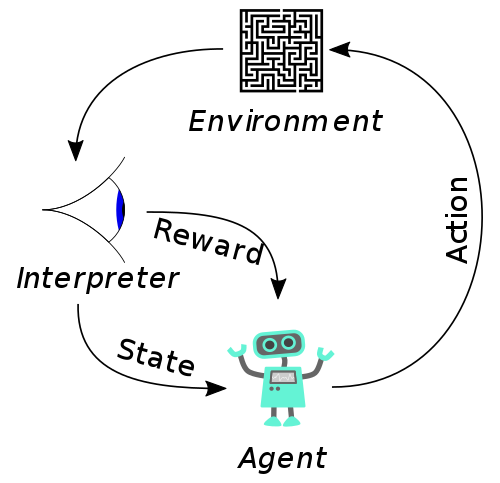
\includegraphics[width=5cm]{figuras/rl}
    \caption{Ilustração de Aprendizado de Reforço}
    \label{fig:rl}
\end{figure}

Aprendizado de Reforço (AR) é uma das grandes áreas que compõe Aprendizado de Máquina (?),
onde são estudados algoritmos que descrevem o comportamento de \textit{agentes} em um \textit{ambiente},
buscando o maior \textit{retorno} por suas ações (ilustrado na figura~\ref{fig:rl}).

Essa definição geral admite aplicação em uma grande quantidade de problemas (?), 
necessitando somente de um ambiente onde o algoritmo possa eficientemente agir e observar a consequência de suas ações. A princípio, não é necessário que o algoritmo seja treinado no mesmo ambiente que ele é ultimamente aplicado, por exemplo, em Robótica, onde o treinamento do algoritmo em um cenário real seria lento e apresentaria riscos para o equipamento, é comum utilizar simulações computacionais do ambiente (que naturalmente introduz outra série de desafios). O maior obstáculo portanto da aplicação de algoritmos de Aprendizado de Reforço tende a ser a quantidade de recursos computacionais necessários para o treinamento.

Pesquisa na área de Aprendizado de Reforço comumente adota jogos eletrônicos como o ambiente para testar seus algoritmos (?), já que estes proporcionam desafios complexos e bem definidos para a análise e comparação de algoritmos, em um ambiente totalmente controlável. Dentro destes, os jogos de estratégia em tempo real (RTS) se destacam por poder envolver um espaço de ação grande e mutável, grande conjunto de estados, temas de planejamento, informação imperfeita e recompensas distantes para as ações dos agentes. Conforme essa tendência, nesse trabalho utilizaremos como estudo de caso um jogo RTS bem simples, criado para a pesquisa de algoritmos de AR.

